\documentclass[11pt,a4paper]{article}

\usepackage[utf8]{inputenc}
\usepackage[LGR,T1]{fontenc}
\usepackage{lmodern}
\usepackage[english,greek]{babel}
\usepackage{microtype}
\usepackage{csquotes}
\usepackage{subcaption}

% ---------- Layout ----------
\usepackage[a4paper,margin=2.5cm]{geometry}
\usepackage{parskip}
\usepackage{titlesec}
\usepackage{xcolor}
\usepackage{booktabs}
\usepackage{enumitem}

% ---------- Math, figures, code ----------
\usepackage{amsmath,amssymb,mathtools}
\usepackage{graphicx}
\usepackage{float}
\usepackage[font=small,labelfont=bf]{caption}
\usepackage{listings}

% ---------- Style ----------
\titleformat{\section}{\Large\bfseries}{\thesection}{0.8em}{}
\titleformat{\subsection}{\large\bfseries}{\thesubsection}{0.8em}{}
\titlespacing*{\section}{0pt}{1.8em}{0.9em}
\titlespacing*{\subsection}{0pt}{1.3em}{0.5em}
\renewcommand{\arraystretch}{1.12}
\setlength{\parskip}{4pt}
\captionsetup{font=small}

\lstset{
    basicstyle=\ttfamily\scriptsize,
    breaklines=true,
    columns=fullflexible,
    showstringspaces=false,
    numbers=left,
    numberstyle=\tiny,
    language=Python,
    frame=single
}

\newcommand{\mur}{\mu_r}
\newcommand{\diff}{\mathrm{diff}}

% ---------- Στοιχεία εξωφύλλου ----------
\newcommand{\studentname}{\textbf{Ονοματεπώνυμο}}
\newcommand{\studentid}{\textbf{Αριθμός Μητρώου}}

\widowpenalty=10000
\clubpenalty=10000
\raggedbottom

\begin{document}

\begin{titlepage}
\thispagestyle{empty}
\centering

{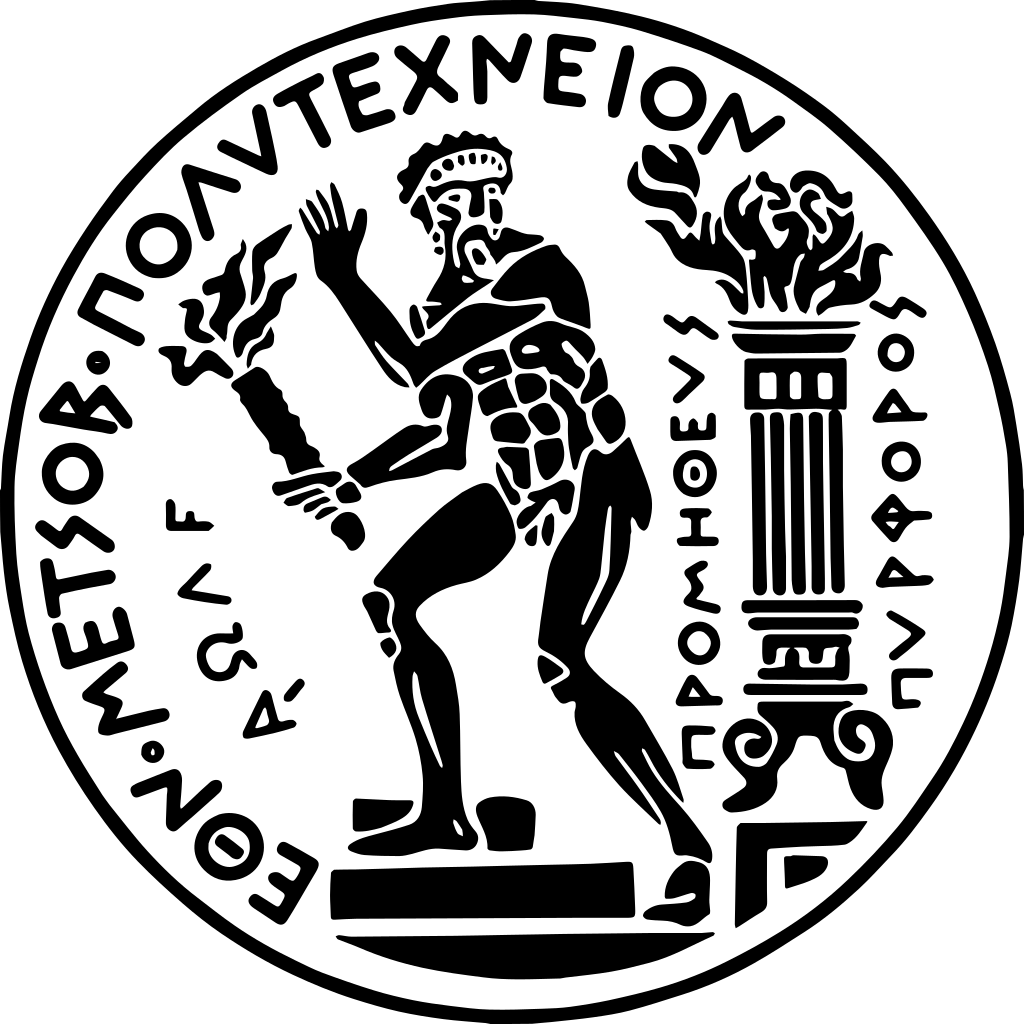
\includegraphics[width=3.5cm]{ntua.png}\\[0.4cm]}

\Large{\textbf{Εθνικό Μετσόβιο Πολυτεχνείο}\\
Σχολή Ηλεκτρολόγων Μηχανικών και Μηχανικών Υπολογιστών}

\vfill

{\huge\bfseries Άσκηση 1}\\[0.6cm]
{\Large Βρόχοι υστέρησης}\vfill

\begin{center}
\large
\renewcommand{\arraystretch}{1.7}
\begin{tabular}{@{}c@{\hspace{2.5em}}c@{}}
    \studentname & \studentid \\
    Διονύσιος Γεώργιος Μουρελάτος & 03122055 \\
    Δημήτριος Λεβογιάννης          & 03122069 \\
    Δήμητρα Καραθάνου              & 03122057 \\
    Ναταλία Λαγού                  & 03122802
\end{tabular}
\end{center}

\vspace{1.2cm}
\today

\vspace*{1cm}
\end{titlepage}

%-------------------
\section{Δεδομένα}

Το αρχείο \textlatin{\texttt{BHloops\_2026\_exercise.xlsx}} περιέχει τέσσερις στήλες ζευγών $(H,B)$ με μονάδες (\textlatin{kA/m}, \textlatin{T}), οι οποίες αντιστοιχούν σε τέσσερις σειρές μετρήσεων βρόχων υστέρησης για 3 δείγματα χαλύβων, μετρημένων στην ίδια διάταξη και υπό τις ίδιες συνθήκες. Κάθε σειρά αποτελείται από 1002 σημεία μέτρησης.

Οι μέγιστες τιμές του εφαρμοζόμενου πεδίου $H_{\max}$ σε κάθε περίπτωση είναι: (1): $1.227$~\textlatin{kA/m}, (2): $1.202$~\textlatin{kA/m}, (3.1): $0.591$~\textlatin{kA/m} και (3.2): $1.182$~\textlatin{kA/m}. Για το δείγμα 3 δίνονται δύο σειρές μετρήσεων, όπου το μέγιστο πεδίο στην περίπτωση (3.1) είναι περίπου το μισό από αυτό των υπολοίπων.

%--------------------------------------------------------------------
\section{Θεωρητικό υπόβαθρο}

\subsection{Βασικές Εξισώσεις}
Όταν ένα υλικό τοποθετείται σε εξωτερικό μαγνητικό πεδίο έντασης $H$ (\textlatin{A/m}), αναπτύσσει εσωτερική \emph{μαγνήτιση} $M$ (\textlatin{A/m}), η οποία εκφράζει τη μαγνητική διπολική ροπή ανά μονάδα όγκου. Η συνολική \emph{μαγνητική επαγωγή} $B$ (\textlatin{T}) δίνεται από τη σχέση:
\begin{equation}
 B = \mu_0 (H + M), \qquad \mu_0 = 4\pi \cdot 10^{-7}\ \mathrm{H/m} \label{eq:B_fund}
\end{equation}
όπου $\mu_0$ είναι η μαγνητική διαπερατότητα του κενού. Από την \eqref{eq:B_fund} και τους ορισμούς της διαπερατότητας και της επιδεκτικότητας προκύπτουν οι εξισώσεις που χρησιμοποιήθηκαν στους υπολογισμούς:
\begin{align}
 M(H) &= \frac{B(H)}{\mu_0} - H \label{eq:M}\\
 \mu(H) &= \frac{B}{H}, \qquad \mu_r(H) = \frac{\mu}{\mu_0}, \qquad \chi(H) = \frac{M}{H} = \mu_r - 1 \label{eq:mu}\\
 \mu_{\diff}(H) &= \frac{dB}{dH}, \qquad \chi_{\diff}(H) = \frac{dM}{dH} = \frac{\mu_{\diff}}{\mu_0} - 1 \label{eq:diff}
\end{align}

\begin{itemize}[nosep]
 \item \textbf{Διαπερατότητα ($\mu$, $\mu_r$) και επιδεκτικότητα ($\chi$):} Η $\mu = B/H$ αντιστοιχεί γεωμετρικά στην κλίση της ευθείας που ενώνει την αρχή των αξόνων $(0,0)$ με το σημείο $(H,B)$, ενώ η $\chi = M/H$ μετρά πόσο έντονα μαγνητίζεται το υλικό από το πεδίο $H$. Επειδή $\chi = \mu_r - 1$ και στα δείγματά μας $\mu_r \sim 500$, οι καμπύλες $\chi(H)$ και $\mu_r(H)$ είναι πρακτικά ίδιες και έχουν τα μέγιστά τους στο ίδιο πεδίο.
 \item \textbf{Διαφορική διαπερατότητα ($\mu_{\diff}$) και επιδεκτικότητα ($\chi_{\diff}$):} Εκφράζουν την τοπική κλίση (εφαπτομένη) των καμπυλών $B(H)$ και $M(H)$ σε κάθε σημείο και δείχνουν πόσο απότομα μεταβάλλεται η μαγνήτιση με το πεδίο. Τα μέγιστά τους εμφανίζονται επίσης στην ίδια τιμή του $H$.
\end{itemize}

\subsection{Παράμετροι του Βρόχου Υστέρησης}
\begin{itemize}[nosep]
 \item \textbf{$B_{\max}$, $M_{\max}$:} Οι μέγιστες τιμές στην κορυφή του βρόχου ($H = H_{\max}$). Όταν το πεδίο δεν επαρκεί για κορεσμό, ο βρόχος είναι ακόρεστος και τα μεγέθη αυτά εξαρτώνται από το επιβαλλόμενο $H_{\max}$ (δεν ταυτίζονται με τις τιμές κορεσμού $B_s, M_s$).
 \item \textbf{Παραμένουσα επαγωγή ($B_r$) και μαγνήτιση ($M_{\mathrm{rem}}$):} Οι τιμές που παραμένουν στο υλικό όταν μηδενιστεί το εξωτερικό πεδίο ($H = 0$), με $M_{\mathrm{rem}} = B_r/\mu_0$.
 \item \textbf{Συνεκτικό πεδίο ($H_c$):} Το αντίθετο πεδίο που απαιτείται για να μηδενιστεί η επαγωγή ($B = 0$, δηλαδή $H_{cB}$). Υπολογίστηκε και το πεδίο όπου $M = 0$ ($H_{ci}$), αλλά διαφέρει λιγότερο από $0.3$~\textlatin{A/m}, οπότε δεν επηρεάζει τα αποτελέσματα.
 \item \textbf{$\mu_{\max}$, $\chi_{\max}$:} Οι μέγιστες τιμές των $B/H$ και $M/H$ στο τεταρτημόριο $H>0,\,B>0$ (και συμμετρικά για $H<0,\,B<0$). Ο περιορισμός αυτός γίνεται επειδή κοντά στο $H \to 0$ (όπου $B \approx \pm B_r \neq 0$) ο λόγος $B/H$ αποκλίνει μαθηματικά ($\to \pm\infty$).
 \item \textbf{$\mu_{\diff,\max}$, $\chi_{\diff,\max}$:} Οι μέγιστες τιμές των κλίσεων $dB/dH$ και $dM/dH$, οι οποίες εμφανίζονται στο πιο απότομο τμήμα του βρόχου, κοντά στο $H_c$.
 \item \textbf{Ενέργεια υστέρησης ($W$):} Το εμβαδόν του βρόχου $W = \oint H\,dB$ (\textlatin{J/m}$^3$), που εκφράζει τις ενεργειακές απώλειες ανά μονάδα όγκου σε κάθε πλήρη κύκλο μαγνήτισης.
\end{itemize}


%--------------------------------------------------------------------
\section{Αποτελέσματα}

\subsection{Πίνακες τιμών και αβεβαιότητες}
Στους Πίνακες~\ref{tab:static} και~\ref{tab:perm} συγκεντρώνονται όλα τα ζητούμενα μεγέθη για τις τέσσερις σειρές μετρήσεων.

\begin{table}[H]\centering
 \begin{tabular}{lcccc}
\toprule
& \textlatin{\#}1 & \textlatin{\#}2 & \textlatin{\#}3.1 & \textlatin{\#}3.2 \\
\midrule
$H_{\max}$ (\textlatin{kA/m}) & 1.227 & 1.202 & 0.591 & 1.182 \\
$B_{\max}$ (\textlatin{T}) & 0.3845 & 0.3738 & 0.2863 & 0.3364 \\
$M_{\max}$ (\textlatin{kA/m}) & 304.8 & 296.3 & 227.2 & 266.5 \\
$M_{\mathrm{rem}}$ (\textlatin{kA/m}) & 105.2 & 56.3 & 71.4 & 79.4 \\
$B_r=\mu_0M_{\mathrm{rem}}$ (\textlatin{T}) & 0.1322 & 0.0708 & 0.0898 & 0.0998 \\
$H_c$ ($B=0$) (\textlatin{A/m}) & 122.7 & 108.0 & 107.4 & 118.1 \\
$B_r/B_{\max}$ & 0.34 & 0.19 & 0.31 & 0.30 \\
$W=\oint H\,dB$ (\textlatin{J/m}$^3$/κύκλο) & 165.8 & 127.0 & 95.6 & 125.8 \\
\bottomrule
\end{tabular}

 \caption{Χαρακτηριστικά μεγέθη των βρόχων.}\label{tab:static}
\end{table}

\begin{table}[H]\centering
 \begin{tabular}{lcccc}
\toprule
& \textlatin{\#}1 & \textlatin{\#}2 & \textlatin{\#}3.1 & \textlatin{\#}3.2 \\
\midrule
$\mu_{\max}$ (\textlatin{mH/m}) & 0.723 & 0.494 & 0.591 & 0.580 \\
$\mu_{r,\max}=\mu_{\max}/\mu_0$ & 575 & 393 & 471 & 462 \\
$H(\mu_{\max})$ (\textlatin{A/m}) & 359 & 467 & 337 & 372 \\
$\mu_{\mathrm{diff,max}}$ (\textlatin{mH/m}) & 1.497 & 0.816 & 1.409 & 1.149 \\
$\mu_{\mathrm{diff,max}}/\mu_0$ & 1191 & 649 & 1122 & 914 \\
$H(\mu_{\mathrm{diff,max}})$ (\textlatin{A/m}) & 131 & 130 & 124 & 133 \\
$\chi_{\max}$ & 574 & 392 & 470 & 461 \\
$H(\chi_{\max})$ (\textlatin{A/m}) & 359 & 467 & 337 & 372 \\
$\chi_{\mathrm{diff,max}}$ & 1190 & 648 & 1121 & 913 \\
$H(\chi_{\mathrm{diff,max}})$ (\textlatin{A/m}) & 131 & 130 & 124 & 133 \\
$B_{\max}/H_{\max}$ (\textlatin{mH/m}) & 0.313 & 0.311 & 0.484 & 0.285 \\
\bottomrule
\end{tabular}

 \caption{Μέγιστες τιμές διαπερατότητας και επιδεκτικότητας και τα πεδία στα οποία εμφανίζονται. Στη γραμμή $B_{\max}/H_{\max}$ δίνεται η διαπερατότητα στην κορυφή του βρόχου.}\label{tab:perm}
\end{table}

\noindent\textbf{Αβεβαιότητες:} Τα $H_c$ και $B_r$ παρουσιάζουν μικρή διαφορά μεταξύ αύξουσας και φθίνουσας διακλάδωσης (έως $4.7$~\textlatin{A/m} και $2.2$~\textlatin{mT} αντίστοιχα). Οι κορυφές των $\mu$ και $\chi$ είναι ομαλές (διαφορά διακλαδώσεων ${<}1\%$, θέση $\pm10$~\textlatin{A/m}). Αντίθετα, λόγω της αριθμητικής παραγώγισης των ακατέργαστων δεδομένων, οι κορυφές των $\mu_\diff$ και $\chi_\diff$ εμφανίζουν θόρυβο: διαφέρουν μεταξύ των δύο διακλαδώσεων κατά έως ${\sim}11\%$ (\textlatin{\#}1: 1257 έναντι 1126, \textlatin{\#}3.1: 1180 έναντι 1063, \textlatin{\#}3.2: 944 έναντι 885, \textlatin{\#}2: 650 έναντι 648) και η θέση τους κατά έως ${\sim}80$~\textlatin{A/m}. Στον πίνακα δίνεται ο μέσος όρος των δύο διακλαδώσεων (με εξομάλυνση οι κορυφές αυτές θα ήταν ελαφρώς χαμηλότερες).

\subsection{Γραφήματα ανά δείγμα}
Τα Σχήματα~\ref{fig:s1}--\ref{fig:s32} απεικονίζουν τα έξι ζητούμενα μεγέθη συναρτήσει του $H$ για κάθε σειρά μετρήσεων (μπλε: αύξουσα διακλάδωση, κόκκινο: φθίνουσα). Τα $\mu_r(H)$ και $\chi(H)$ αποκόπτονται κοντά στο $H=0$, όπου ο λόγος $B/H$ αποκλίνει.

\begin{figure}[!htbp]\centering
 \includegraphics[width=0.92\textwidth]{figs/sample_1.pdf}
 \caption{Δείγμα \textlatin{\#}1: $B$, $M$, $\mu_r=\mu/\mu_0$, $\mu_{\diff}/\mu_0$, $\chi$, $\chi_{\diff}$ συναρτήσει του $H$.}\label{fig:s1}
\end{figure}
\begin{figure}[!htbp]\centering
 \includegraphics[width=0.92\textwidth]{figs/sample_2.pdf}
 \caption{Δείγμα \textlatin{\#}2.}\label{fig:s2}
\end{figure}
\begin{figure}[!htbp]\centering
 \includegraphics[width=0.92\textwidth]{figs/sample_3.1.pdf}
 \caption{Δείγμα \textlatin{\#}3.1 (μικρότερος βρόχος, $H_{\max}=0.59$~\textlatin{kA/m}).}\label{fig:s31}
\end{figure}
\begin{figure}[!htbp]\centering
 \includegraphics[width=0.92\textwidth]{figs/sample_3.2.pdf}
 \caption{Δείγμα \textlatin{\#}3.2 ($H_{\max}=1.18$~\textlatin{kA/m}).}\label{fig:s32}
\end{figure}

%--------------------------------------------------------------------
\clearpage
\section{Σύγκριση και σχολιασμός}

\subsection{Γενικά χαρακτηριστικά}
\begin{itemize}
 \item \textbf{Μαλακά, μη κορεσμένα υλικά:} Με βάση το κριτήριο $H_c < 1$~\textlatin{kA/m}, και τα τρία δείγματα είναι \textbf{μαλακά μαγνητικά υλικά}, αφού τα συνεκτικά τους πεδία ($H_c \approx 107$--$123$~\textlatin{A/m}) είναι περίπου δέκα φορές μικρότερα από το όριο αυτό. Επίσης, κανένας βρόχος δεν φτάνει σε κορεσμό: η μέγιστη μαγνήτιση είναι πολύ μικρότερη από την τυπική τιμή κορεσμού του σιδήρου ($M_s \approx 1.7$~\textlatin{MA/m}), ενώ στα άκρα των βρόχων η διαφορική διαπερατότητα παραμένει $\mu_\diff/\mu_0 \approx 30$--$60$ αντί να τείνει στο $1$. Επομένως, το $B_{\max}$ εξαρτάται από το εφαρμοζόμενο πεδίο και δεν είναι $B_s$.
 \item \textbf{Μορφή βρόχου:} Και οι τέσσερις καμπύλες έχουν σιγμοειδή μορφή (Σχ.~\ref{fig:cmpBM}), με απότομη μεταβολή γύρω από το $H_c$ και μια χαρακτηριστική γωνία στα $300$--$500$~\textlatin{A/m}. Το απότομο κεντρικό τμήμα οφείλεται στην ταχεία κίνηση των μαγνητικών τοιχωμάτων, ενώ το ανώτερο τμήμα μικρότερης κλίσης (χαμηλή $\mu_\diff$) αντιστοιχεί στη σταδιακή περιστροφή της μαγνήτισης προς τη διεύθυνση του πεδίου.
\end{itemize}

\begin{figure}[!htbp]\centering
 \begin{subfigure}{.49\textwidth}\includegraphics[width=\textwidth]{figs/cmp_B.pdf}\caption{$B(H)$}\end{subfigure}
 \begin{subfigure}{.49\textwidth}\includegraphics[width=\textwidth]{figs/cmp_M.pdf}\caption{$M(H)$}\end{subfigure}
 \caption{Σύγκριση των τεσσάρων βρόχων υστέρησης.}\label{fig:cmpBM}
\end{figure}

\subsection{Σύγκριση των δειγμάτων \textlatin{\#}1, \textlatin{\#}2 και \textlatin{\#}3}
\begin{itemize}
 \item \textbf{Δείγμα \textlatin{\#}1:} Έχει τον πιο «τετράγωνο» βρόχο, με τη μεγαλύτερη παραμένουσα επαγωγή ($B_r/B_{\max}=0.34$), τις υψηλότερες τιμές διαπερατότητας ($\mu_{r,\max}, \mu_{\diff,\max}$) και την πιο στενή, οξεία κορυφή στη $\mu_\diff$ (Σχ.~\ref{fig:cmpmu}). Αυτό δείχνει ότι η αναστροφή της μαγνήτισης γίνεται απότομα σε στενό εύρος πεδίων. Παράλληλα, έχει το μεγαλύτερο $H_c$ και το μεγαλύτερο εμβαδόν $W$, άρα και τις μεγαλύτερες απώλειες ανά κύκλο.
 \item \textbf{Δείγμα \textlatin{\#}2:} Παρότι φτάνει σχεδόν την ίδια μέγιστη επαγωγή $B_{\max}$ με το \textlatin{\#}1, ο βρόχος του είναι πιο λοξός και στενός, με σχεδόν τη μισή παραμένουσα επαγωγή ($B_r/B_{\max}=0.19$) και μια χαμηλή, πλατιά κορυφή στη $\mu_\diff$. Η πλατιά αυτή κορυφή δείχνει ότι η αναστροφή των μαγνητικών περιοχών γίνεται πιο σταδιακά σε μεγαλύτερο εύρος πεδίων (λόγω διαφορετικής μικροδομής, εσωτερικών τάσεων ή γεωμετρίας μέτρησης). Έτσι, έχει τη χαμηλότερη διαπερατότητα αλλά και αισθητά μικρότερες απώλειες $W$ από το \textlatin{\#}1.
 \item \textbf{Δείγμα \textlatin{\#}3 (\textlatin{\#}3.2):} Βρίσκεται ανάμεσα στα δύο προηγούμενα ως προς το $H_c$, το $B_r$ και τη διαπερατότητα, ενώ έχει χαμηλές απώλειες $W$ (σχεδόν ίσες με του \textlatin{\#}2). Ξεχωρίζει όμως επειδή παρουσιάζει μικρότερο $B_{\max}$ και $M_{\max}$ στο ίδιο πεδίο, κάτι που υποδηλώνει είτε χαμηλότερη μαγνήτιση κορεσμού $M_s$ (διαφορετική σύσταση χάλυβα) είτε πιο αργή προσέγγιση του κορεσμού.
 \item \textbf{Συνολικά:} Στα $H_c$, $B_r$, $\mu_{r,\max}$ και $\mu_{\diff,\max}$ η κατάταξη είναι \textlatin{\#}1 $>$ \textlatin{\#}3.2 $>$ \textlatin{\#}2, ενώ στις απώλειες $W$ είναι \textlatin{\#}1 $>$ \textlatin{\#}2 $\approx$ \textlatin{\#}3.2. Παρατηρείται δηλαδή ότι το δείγμα με την πιο απότομη αναστροφή (\textlatin{\#}1) συνδυάζει την υψηλότερη διαπερατότητα με τις μεγαλύτερες απώλειες.
\end{itemize}

\begin{figure}[!htbp]\centering
 \begin{subfigure}{.49\textwidth}\includegraphics[width=\textwidth]{figs/cmp_mu.pdf}\caption{$\mu_r(H)$}\end{subfigure}
 \begin{subfigure}{.49\textwidth}\includegraphics[width=\textwidth]{figs/cmp_chi.pdf}\caption{$\chi(H)$}\end{subfigure}
 \begin{subfigure}{.49\textwidth}\includegraphics[width=\textwidth]{figs/cmp_mud.pdf}\caption{$\mu_{\diff}/\mu_0$}\end{subfigure}
 \begin{subfigure}{.49\textwidth}\includegraphics[width=\textwidth]{figs/cmp_chid.pdf}\caption{$\chi_{\diff}(H)$}\end{subfigure}
 \caption{Σύγκριση διαπερατότητας και επιδεκτικότητας.}\label{fig:cmpmu}
\end{figure}

\subsection{Σύγκριση \textlatin{\#}3.1 και \textlatin{\#}3.2}
Οι μετρήσεις \textlatin{\#}3.1 και \textlatin{\#}3.2 αφορούν το ίδιο δείγμα χάλυβα, με τη διαφορά ότι στο \textlatin{\#}3.1 εφαρμόζεται το μισό μέγιστο πεδίο ($H_{\max} \approx 591$~\textlatin{A/m} έναντι $1182$~\textlatin{A/m}). Επομένως, το \textlatin{\#}3.1 αποτελεί έναν μικρότερο, εσωτερικό βρόχο του \textlatin{\#}3.2:
\begin{itemize}
 \item \textbf{Παρόμοια συμπεριφορά στο κεντρικό τμήμα:} Η απότομη άνοδος της καμπύλης $B(H)$ συμβαίνει γύρω στα $120$--$130$~\textlatin{A/m} και ολοκληρώνεται περίπου στα $400$--$500$~\textlatin{A/m}. Επειδή το \textlatin{\#}3.1 φτάνει μέχρι τα $591$~\textlatin{A/m}, προλαβαίνει να διανύσει ολόκληρο αυτό το απότομο τμήμα και απλώς σταματά νωρίτερα. Γι' αυτόν τον λόγο, οι δύο βρόχοι επικαλύπτονται για $|H| < 590$~\textlatin{A/m}, και τα μεγέθη $H_c$, $\mu_{r,\max}$, $B_r/B_{\max}$ καθώς και η θέση της κορυφής της $\mu_\diff$ παραμένουν σχεδόν ίδια.
 \item \textbf{Μικρότερος λόγος $B_{\max}/H_{\max}$ στον μεγάλο βρόχο:} Στο \textlatin{\#}3.2 το μέγιστο πεδίο $H_{\max}$ διπλασιάζεται, όμως η καμπύλη $B(H)$ έχει ήδη αρχίσει να οριζοντιώνεται, οπότε το $B_{\max}$ αυξάνεται ελάχιστα. Έτσι, ο λόγος $B_{\max}/H_{\max}$ στην κορυφή μειώνεται από $0.48$ σε $0.28$~\textlatin{mH/m}, σχεδόν ο μισός.
\end{itemize}


%--------------------------------------------------------------------
\section{Συμπεράσματα}
Και τα τρία δείγματα συμπεριφέρονται ως μαλακά μαγνητικά υλικά ($H_c \approx 107$--$123$~\textlatin{A/m} $\ll 1$~\textlatin{kA/m}) και δεν φτάνουν σε κορεσμό. Το \textbf{δείγμα \textlatin{\#}1} έχει τον πιο τετράγωνο βρόχο και τη μεγαλύτερη διαπερατότητα, αλλά και τις μεγαλύτερες απώλειες ανά κύκλο. Το \textbf{δείγμα \textlatin{\#}2} έχει τον πιο λοξό βρόχο, τη χαμηλότερη διαπερατότητα και χαμηλές απώλειες, ενώ το \textbf{δείγμα \textlatin{\#}3} βρίσκεται ενδιάμεσα με χαμηλότερη επαγωγή στο ίδιο πεδίο. Τέλος, η σύγκριση \textbf{\textlatin{\#}3.1} και \textbf{\textlatin{\#}3.2} δείχνει ότι εφόσον το μέγιστο πεδίο ξεπερνά την απότομη περιοχή αναστροφής, οι βασικές παράμετροι ($H_c$, $B_r/B_{\max}$ και η θέση της κορυφής της $\mu_\diff$) μεταβάλλονται ελάχιστα, ενώ η διαπερατότητα κορυφής $B_{\max}/H_{\max}$ είναι υψηλότερη στον μικρότερο βρόχο.


\end{document}